\section{Test of client-server communication}
To be certain that our client server communication works as it should, we will do both "real-life" practical tests and black-box testing, e.g. making sure the client and server behaves as it should on different occasions.

\subsection{Connection between client and server}
To make sure that the client(s) can connect to our server we have tested it in the following ways.
\begin{itemize}
	\item From local host, we started the server from the IntelliJ IDE and afterwards we started the client from Android Studio and connected to the server. In IntelliJ we could see that the server accepted the connection. Which is shown in 
		\begin{figure}[h!]
  \centering
	    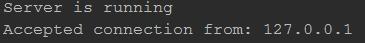
\includegraphics[width=0.6\textwidth]{figures/serverrunning.png}
    \caption{Server running and accepting connection}
    \label{fig:serverrunning}
\end{figure}
	\item From seperate clients, we started the server as with the local host testing, but to test the targetted device, e.g smartphones, we downloaded the application to 7 smartphones and connected them to the server. It showed in IntelliJ's prompt window that the connections from each smartphone were successful.
\end{itemize}

\subsection{Message received matches the message sent}
To be certain the longitude, latitude and speed that is sent is received correctly on the server. We did the following test:
\begin{itemize}
	\item We gave the emulator in Android Studio a specific longitude and latitude and then used the application to send the data to the server. In IntelliJ's prompt window we got the following information displayed in \figref{fig:datasentfromclienttoserver}. Which confirms that the message sent from the client is received correctly on the server.
	\begin{figure}[h!]
  \centering
    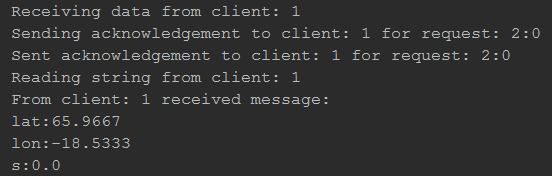
\includegraphics[width=0.8\textwidth]{figures/datasentfromclienttoserver.png}
    \caption{Data received on the server from the client}
    \label{fig:datasentfromclienttoserver}
\end{figure}
	\item \todo{Use mortens phone to get a proper speed test instead of the 0.0 from the emulator}
\end{itemize}

\subsection{Is the three-way handshake condition met }
In 

\subsection{GPS location and speed}
The location of the client and the speed it is moving at has been tested in a car with one person driving the car and another using a smartphone, where the smartphone displays the current speed and the location after a click on a button. The speed was compared to the car's speedometer which matched and the GPS location that was shown was later checked on a map, where the locations given by the smartphone also were correct.

\todo{Add more tests to client-server!}